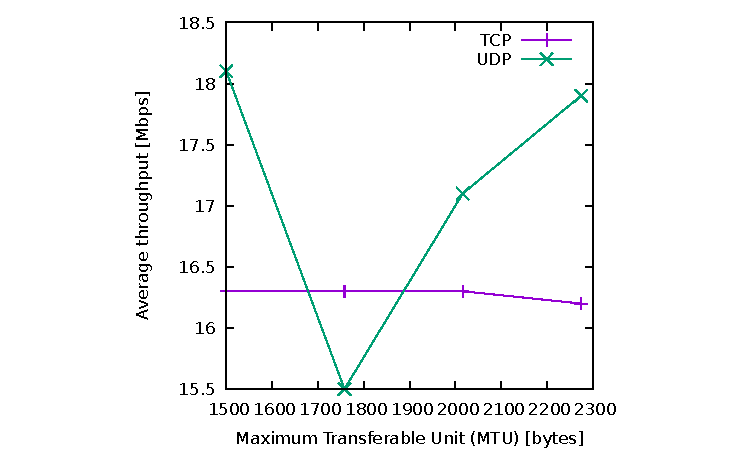
\includegraphics[width=0.5\textwidth]{traces/L3-5-2-tput.pdf}

UDP shows a very clear drop in throughput when increasing the frame length over 1452 bytes. While the first trace (/traces/L3-5-2.udp.1500.pcap) just shows regular UDP datagrams, the following three dumps show IPv6 fragmentation. For example in traces/L3.5.2.udp.1758.pcap, the iperf client first tries to send a UDP packet of length 1772 (packet 1). An ICMPv6 message indicating this packet exceeded the MTU is sent back (packet 2). Each following frame containing 1710 bytes of application data is now divided across two packets (e.g. packet 3+4) each respecting the Path MTU. First an IPv6 fragment is filled with as much data as the path MTU will allow. The remaining data, along with the UDP header is sent in a second packet. This means each 1710 byte frame now requires two sets of layer 2 and 3 headers, significantly increasing the overhead (relative to the amount of application data) and explaining the drop in throughput. We can calculate the relative overhead (assuming Ethernet at layer 2). The 1458 byte frames had 14 (ethernet) + 40 (IPv6) + 8 (UDP) = 62 bytes of headers, meaning ~4.1\% of transmitted data was overhead. For the 1710 byte frames this becomes 2 * 14 (ethernet) + 2 * 48 (IPv6 with fragmentation header) + 8 (UDP) = 132 bytes of headers, leading to ~7.2\% overhead. \\ \\ For further increases in frame length, the throughput starts to rise again. Each 1710 byte frame was divded into parts of 1448 and 262 bytes and each sent in a separate packet. Each packet could contain up to 1452 bytes with this path MTU. For the 1968 and 2226 frame lengths, each frame is still fragmented into only two parts, but the second fragment is bigger (respectively 520 and 778 bytes of application data). By sending fuller packets, the relative overhead decreases and the throughput increases. \\ \\
For TCP the throughput remains stable while increasing the wireless link's MTU. In UDP's case the fragmentation was triggered by also increasing the frame length. For TCP no such option exists. Even if we set the Maximum Segment Size (MSS) to something exceeding the Path MTU, the kernel will first discover the Path MTU and lower the segment size to not exceed the Path MTU. In each of the traces the data is sent to the iperf server in packets of 1514 bytes. Having an MTU higher than the actual packet size somewhere in the data path makes no difference, there is no real difference between the four test cases with TCP.
